\documentclass [12pt, a4paper, english, brazil, oneside, chapter=TITLE, section=TITLE]{abntex2}
% Para impressão use doubleside
% ---
% Arquivo com  a formatação é lido aqui. Não deve ser modificado
% ---
% ---
% Arquivo com a formatação do TCC.
% Este arquivo não deve ser modificado.
% ---
\usepackage[utf8]{inputenc}
\usepackage[T1]{fontenc}
\usepackage{amsmath}
\usepackage{amssymb,amsfonts,textcomp}
\usepackage{color}
\usepackage{array}
\usepackage{supertabular}
\usepackage{listings}         % Para as linguagens de programação
\usepackage{lastpage}		  % Usado pela Ficha catalográfica
\usepackage{indentfirst}	  % Indenta o primeiro parágrafo de cada seção.
\usepackage{hhline}
\usepackage{hyperref}
\usepackage[pdftex]{graphicx}
\usepackage{float}
\graphicspath{ {./figuras/} }

% retira as mensagens de aviso do pacote Glossaries
\let\printglossary\relax
\let\theglossary\relax
\let\endtheglossary\relax
% coloca Seções em maiúsculas sem negrito no Sumário
\makeatletter
\let\oldcontentsline\contentsline
\def\contentsline#1#2{%
  \expandafter\ifx\csname l@#1\endcsname\l@section
    \expandafter\@firstoftwo
  \else
    \expandafter\@secondoftwo
  \fi
  {%
    \oldcontentsline{#1}{\normalfont\MakeTextUppercase{#2}}%
  }{%
    \oldcontentsline{#1}{#2}%
  }%
}
\makeatother
% ---
% Pacotes glossaries
% ---
\usepackage[subentrycounter,seeautonumberlist,nonumberlist=true]{glossaries}
% para usar o xindy ao invés do makeindex:
%\usepackage[xindy={language=portuguese},subentrycounter,seeautonumberlist,nonumberlist=true]{glossaries}
% ---
% Citações de referências no formato alfabético e negrito
\usepackage[alf, abnt-emphasize=bf]{abntex2cite} 
% Margens definidas em 25 mm para uso como documento em PDF
% Para imprimir use as seguintes margens:
% \usepackage[left=30mm, top=30mm, right=20 mm, bottom=20mm] {geometry}

\usepackage[margin=25 mm]{geometry}
%---
% O arquivo com o nome dos alunos e dos orientadores é lido aqui.
% Atualizar diretamente no arquivo
%---
%%%%%%%%%%%%%%%%%%%%%%%%%%%%%%%%%%%%%%%%%%%%%%%%%%%%%%%%%%%%%
% Definições de Macros utilizadas no TCC - ATUALIZE AQUI
%%%%%%%%%%%%%%%%%%%%%%%%%%%%%%%%%%%%%%%%%%%%%%%%%%%%%%%%%%%%%
\instituicao{UNIVERSIDADE FEDERAL DO RIO DE JANEIRO
\par
INSTITUTO DE COMPUTAÇÃO
\par
CURSO DE BACHARELADO EM CIÊNCIA DA COMPUTAÇÃO}
\title{HARDENING DE APLICAÇÓES WEB: Um panorama e soluções}
\autor{Daigoro Alencar de Oliveira \\ Henrique Vermelho de Toledo}
\orientador{Prof. Paulo Henrique Rodrigues Aguiar }
\coorientador{Prof. Cláudio Miceli Farias}
\local{RIO DE JANEIRO}
\data{2022}
\preambulo{Trabalho de conclusão de curso de graduação apresentado ao Instituto de Computação da Universidade Federal do Rio de Janeiro como parte dos requisitos para obtenção do grau de Bacharel em Ciência da Computação.}

%%%%%%%%%%%%%%%%%%%%%%%%%%%%%%%%%%%%%%%%%%%%%%%%%%%%%%%%%%%
% Corrige a fonte dos capítulos, seções, resumos, etc.
%%%%%%%%%%%%%%%%%%%%%%%%%%%%%%%%%%%%%%%%%%%%%%%%%%%%%%%%%%%

\renewcommand{\ABNTEXchapterfont}{\bfseries \rmfamily}  % Capítulos em Bold e Maiúsculas
\renewcommand{\ABNTEXchapterfontsize}{\normalsize}
\renewcommand{\ABNTEXsectionfont}{\rmfamily}            %  Seções em  Maiúsculas apenas
\renewcommand{\ABNTEXsectionfontsize}{\normalsize}
\renewcommand{\ABNTEXsubsectionfont}{\bfseries}         % Subseções em Bold apenas
\renewcommand{\ABNTEXsubsectionfontsize}{\normalsize}
\renewcommand{\lstlistingname}{Código}                  % Nome para os códigos no texto
\renewcommand{\lstlistlistingname}{Lista de \lstlistingname s}
\makeatletter                                          % Configura a linha da lista de códigos
\renewcommand\l@lstlisting[2]{{\normalfont\@dottedtocline{1}{1.5em}{2em}{Código~#1}{#2}}}
\makeatother
\usepackage{url16023}  % para retirar < e > da URL nas referências.
%%%%%%%%%%%%%%%%%%%%%%%%%%%%%%%%%%%%%%%%%%%%%%%%%%%%%%%%%%%
% Criação de quadros com numeração
%%%%%%%%%%%%%%%%%%%%%%%%%%%%%%%%%%%%%%%%%%%%%%%%%%%%%%%%%%%
\newcommand{\quadroname}{Quadro}
% \newcommand{\listofquadrosname}{Lista de quadros}

% \newfloat[chapter]{quadro}{loq}{\quadroname}
\newlistof{listofquadros}{loq}{\listofquadrosname}
\newlistentry{quadro}{loq}{0}
%%%%%%%%%%%%%%%%%%%%%%%%%%%%%%%%%%%%%%%%%%%%%%%%%%%%%%%%%%%
% configurações para atender às regras da ABNT
%%%%%%%%%%%%%%%%%%%%%%%%%%%%%%%%%%%%%%%%%%%%%%%%%%%%%%%%%%%
\setfloatadjustment{quadro}{\centering}
\counterwithout{quadro}{chapter}
\renewcommand{\cftquadroname}{\quadroname\space} 
\renewcommand*{\cftquadroaftersnum}{\hfill--\hfill}
%---
% Configuração de posicionamento padrão
%---
\setfloatlocations{quadro}{hbtp}
%---
% Para ajudar nas tabelas e quadros
%---
\makeatletter
\newcommand\arraybslash{\let\\\@arraycr}
\makeatother
%%%%%%%%%%%%%%%%%%%%%%%%%%%%%%%%%%%%%%%%%%%%%%%%%%%%%%%
% Redefine a macro para imprimir a capa 
%%%%%%%%%%%%%%%%%%%%%%%%%%%%%%%%%%%%%%%%%%%%%%%%%%%%%%%
\renewcommand{\imprimircapa}{%
\begin{capa}%
\center
\imprimirinstituicao
\par
\vspace*{1cm}
\MakeUppercase{\imprimirautor}
\vfill
\begin{center}
\imprimirtitulo
\end{center}
\vfill
\imprimirlocal
\par
\imprimirdata
\vspace*{1cm}
\end{capa}
}
%%%%%%%%%%%%%%%%%%%%%%%%%%%%%%%%%%%%%%%%%%%%%%%%%%%%%%%
% Redefine a macro para imprimir a folho de rosto
%%%%%%%%%%%%%%%%%%%%%%%%%%%%%%%%%%%%%%%%%%%%%%%%%%%%%%%
\renewcommand{\imprimirfolhaderosto}{%
\begin{capa}%
\center
\par
\vspace*{1cm}
\MakeUppercase{\imprimirautor}
\vfill
\begin{center}
\imprimirtitulo
\end{center}
\vfill
\hspace*{\fill}\parbox[b]{.5\textwidth}{%
        \linespread{1}\selectfont
\imprimirpreambulo
}
\vfill
\flushright
Orientador: \imprimirorientador\\

Co-orientador: \imprimircoorientador\\
\vfill
\begin{center}
\large\imprimirlocal
\par
\large\imprimirdata
\vspace*{1cm}
\end{center}
\end{capa}
}
%%%%%%%%%%%%%%%%%%%%%%%%%%%%%%%%%%%%%%%%%%%%%%%%%%%%%%%
% Informações do PDF inseridas automaticamente
% Atualizar apenas as palavras-chave se necessário
% Não modificar as cores dos links e referências
%%%%%%%%%%%%%%%%%%%%%%%%%%%%%%%%%%%%%%%%%%%%%%%%%%%%%%%
\makeatletter
\hypersetup{
pdftitle={\@title},
pdfauthor={\@author},
pdfsubject={\imprimirpreambulo},
pdfkeywords={MONOGRAFIA}{CIÊNCIA DA COMPUTAÇÃO}{DCC-UFRJ},
pdfcreator={LaTeX with abnTeX2},
colorlinks=true,
linkcolor=black,
citecolor=black,
urlcolor=black
}
\makeatother
%%%%%%%%%%%%%%%%%%%%%%%%%%%%%%%%%%%%%%%%%%%%%%%%%%%%
% Definição das Linguagens de Programação
%%%%%%%%%%%%%%%%%%%%%%%%%%%%%%%%%%%%%%%%%%%%%%%%%%%%
\definecolor{dkgreen}{rgb}{0,0.6,0}
\definecolor{gray}{rgb}{0.5,0.5,0.5}
\definecolor{purple}{rgb}{0.8,0,0.3}
\definecolor{orange}{rgb}{1,0.4,0}
\definecolor{lightlightgray}{rgb}{.95,.95,.95}
\definecolor{lightgray}{rgb}{.9,.9,.9}
\definecolor{lightgray2}{rgb}{.85,.85,.85}
\definecolor{darkgray}{rgb}{.4,.4,.4}
%---
% Comando para inserir a listagem de código, tem 4 parâmetros
% Linguagem, Caption, Label, Nome do Arquivo
%---
\newcommand{\includecode}[4][C]{\mbox{\lstinputlisting[caption=#2, label=#3, escapechar=, style=custom#1]{#4}}}

%---
%Define características em comum e numeração sequencial 
%---
\lstset{numberbychapter=false,framexleftmargin=5mm,  frame=shadowbox, rulesepcolor=\color{gray}}
%---
% A leitura da formatação das linguagens é feita aqui. 
% Modifique diretamente no arquivo.
%
%%%%%%%%%%%%%%%%%%%%%%%%%%%%%%%%%%%%%%%%%%%%%%%%%%%%
% Aqui você pode personalizar a linguagem C  
%%%%%%%%%%%%%%%%%%%%%%%%%%%%%%%%%%%%%%%%%%%%%%%%%%%%
\lstdefinestyle{customC}{
      language = C,
      breaklines=true,
      basicstyle=\footnotesize\ttfamily,
      keywordstyle=\bfseries\color{blue},
      commentstyle=\itshape\color{purple},
      identifierstyle=\color{black},
      stringstyle=\color{orange},
      showstringspaces=false}

%%%%%%%%%%%%%%%%%%%%%%%%%%%%%%%%%%%%%%%%%%%%%%%%%%%%
% Aqui você pode personalizar a linguagem Java 
%%%%%%%%%%%%%%%%%%%%%%%%%%%%%%%%%%%%%%%%%%%%%%%%%%%%       
\lstdefinestyle{customJava}{
      language = Java,
      breaklines=true,
      basicstyle=\footnotesize\ttfamily,
      keywordstyle=\bfseries\color{blue},
      commentstyle=\itshape\color{purple},
      identifierstyle=\color{black},
      stringstyle=\color{orange},
      showstringspaces=false}
%%%%%%%%%%%%%%%%%%%%%%%%%%%%%%%%%%%%%%%%%%%%%%%%%%%%
% Aqui você pode personalizar a linguagem C++
%%%%%%%%%%%%%%%%%%%%%%%%%%%%%%%%%%%%%%%%%%%%%%%%%%%%  
\lstdefinestyle{customC++}{
      language = C++,
      breaklines=true,
      basicstyle=\footnotesize\ttfamily,
      keywordstyle=\bfseries\color{blue},
      commentstyle=\itshape\color{purple},
      identifierstyle=\color{black},
      stringstyle=\color{orange},
      showstringspaces=false}
%%%%%%%%%%%%%%%%%%%%%%%%%%%%%%%%%%%%%%%%%%%%%%%%%%%%
% Aqui você pode personalizar a linguagem Javascript
%%%%%%%%%%%%%%%%%%%%%%%%%%%%%%%%%%%%%%%%%%%%%%%%%%%%        
\lstdefinestyle{customJavaScript}{
      language = JavaScript,
      breaklines=true,
      basicstyle=\footnotesize\ttfamily,
      keywordstyle=\bfseries\color{blue},
      commentstyle=\itshape\color{purple},
      identifierstyle=\color{black},
      stringstyle=\color{orange},
      showstringspaces=false}
      
% Javascript
\lstdefinelanguage{JavaScript}{
    aboveskip=15pt,
    keywords={typeof, new, true, false, catch, function, return, null, catch, switch, var, if, in, while, do, else, case, break},
    keywordstyle=\color{blue}\bfseries,
    ndkeywords={class, export, boolean, throw, implements, import, this},
    ndkeywordstyle=\color{darkgray}\bfseries,
    identifierstyle=\color{black},
    sensitive=false,
    comment=[l]{//},
    morecomment=[s]{/*}{*/},
    commentstyle=\color{purple}\ttfamily,
    stringstyle=\color{red}\ttfamily,
    morestring=[b]',
    morestring=[b]",
    rulecolor=\color{lightgray2},
    breaklines=true,
    basicstyle=\footnotesize\ttfamily,
    frame=single,
    backgroundcolor=\color{lightlightgray}
}
%%%%%%%%%%%%%%%%%%%%%%%%%%%%%%%%%%%%%%%%%%%%%%%%%%%%
% Aqui você pode personalizar o formato JSON
%%%%%%%%%%%%%%%%%%%%%%%%%%%%%%%%%%%%%%%%%%%%%%%%%%%%        
\lstdefinestyle{customJSON}{
      language = JSON,
      breaklines=true,
      basicstyle=\footnotesize\ttfamily,
      keywordstyle=\bfseries\color{blue},
      commentstyle=\itshape\color{purple},
      identifierstyle=\color{black},
      stringstyle=\color{orange},
      showstringspaces=false}
      
% JSON
\lstdefinelanguage{JSON}{
    aboveskip=15pt,
    string=[s]{"}{"},
    stringstyle=\color{blue},
    comment=[l]{:},
    commentstyle=\color{black},
    rulecolor=\color{lightgray2},
    breaklines=true,
    basicstyle=\footnotesize\ttfamily,
    frame=single,
    backgroundcolor=\color{lightlightgray}
}
%%%%%%%%%%%%%%%%%%%%%%%%%%%%%%%%%%%%%%%%%%%%%%%%%%%%
% Aqui você pode personalizar a linguagem de montagem do SAPIENS
%%%%%%%%%%%%%%%%%%%%%%%%%%%%%%%%%%%%%%%%%%%%%%%%%%%%       
\lstdefinestyle{customSapiens}{
      language = Sapiens,
      breaklines=true,
      basicstyle=\footnotesize\ttfamily,
      keywordstyle=\bfseries\color{blue},
      commentstyle=\itshape\color{purple},
      identifierstyle=\color{black},
      stringstyle=\color{orange},
      showstringspaces=false}

\lstdefinestyle{Python}{
    language=Python,
    backgroundcolor=\color{backcolour},   
    commentstyle=\color{codegreen},
    keywordstyle=\color{magenta},
    numberstyle=\tiny\color{codegray},
    stringstyle=\color{codepurple},
    basicstyle=\ttfamily\footnotesize,
    breakatwhitespace=false,         
    breaklines=true,                 
    captionpos=b,                    
    keepspaces=true,                 
    numbers=left,                    
    numbersep=5pt,                  
    showstringspaces=false,
}
% Linguagem de Montagem    
\lstdefinelanguage{Sapiens}{
    aboveskip=15pt,
    keywordstyle=\color{blue}\bfseries,
    comment=[l]{;},
    commentstyle=\color{purple},
    rulecolor=\color{lightgray2},
    breaklines=true,
    basicstyle=\footnotesize\ttfamily,
    frame=single,
    backgroundcolor=\color{lightlightgray},
    language=[x86masm]Assembler,
    morekeywords={DB, DS, DW, JN, JSR, LDA, ORG, STA, STS, TRAP}
}
     
%---
% FIM
%---
% ---
% GLOSSÁRIO
% ---
\makeglossaries
% ---
% Entradas do glossário
% ---
\newglossaryentry{componente}{
               name={componente},
               plural={componentes},
%               parent=pai,
               description={descrição da entrada componente} }
 
\newglossaryentry{equilibrio}{
                name={equilíbrio da configuração},
                see=[veja também]{componente},
                description={consistência entre os \glspl{componente}}
                }

\newglossaryentry{latex}{
                name={LaTeX},
                description={ferramenta de computador para autoria de documentos criada por D. E. Knuth} }

\newglossaryentry{abntex2}{
                name={abnTeX2},
                see=latex,
                description={suíte para LaTeX que atende os requisitos das
                normas da ABNT para elaboração de documentos técnicos e científicos brasileiros} }
                
\newglossaryentry{maths}
{
    name=matemática,
    description={Matemática é o que os matemáticos fazem}
}

\newglossaryentry{formula}
{
        name=formula,
        description={Uma expressão matemática}
}
 
\newacronym{mdc}{MDC}{Maior Divisor Comum}
 
\newacronym{mmc}{MMC}{Mínimo Múltipo Comum}


% ---
%\item [Palavra] Significado da palavra

%\item [Palavra 2] Significado da palavra 2
% ---
%%%%%%%%%%%%%%%%%%%%%%%%%%%%%%%%%%%%%%%%%%%%%%%%%%%%%%%%%%%%
% I N I C I O  D O  D O C U M E N T O
%%%%%%%%%%%%%%%%%%%%%%%%%%%%%%%%%%%%%%%%%%%%%%%%%%%%%%%%%%%%
\begin{document}
\pretextual

%%%%%%%%%%%%%%%%%%%%%%%%%%%%%%%%%%%%%%%%%%%%%%%%%%%%%%%%%%%%
% C A P A (OBRIGATÓRIO)
%%%%%%%%%%%%%%%%%%%%%%%%%%%%%%%%%%%%%%%%%%%%%%%%%%%%%%%%%%%%

\setcounter{page}{1}
\imprimircapa

%%%%%%%%%%%%%%%%%%%%%%%%%%%%%%%%%%%%%%%%%%%%%%%%%%%%%%%%%%%%
% F O L H A  D E  R O S T O  (OBRIGATÓRIO)
%%%%%%%%%%%%%%%%%%%%%%%%%%%%%%%%%%%%%%%%%%%%%%%%%%%%%%%%%%%%

\imprimirfolhaderosto

%%%%%%%%%%%%%%%%%%%%%%%%%%%%%%%%%%%%%%%%%%%%%%%%%%%%%%%%%%%%
% F I C H A   C A T A L O G R Á F I A  (OBRIGATÓRIO)
%%%%%%%%%%%%%%%%%%%%%%%%%%%%%%%%%%%%%%%%%%%%%%%%%%%%%%%%%%%%
% Ficha catalográfica (obrigatório)
% Para elaborar a ficha catalográfica siga as instruções em
% http://fichacatalografica.sibi.ufrj.br/}
%%%%%%%%%%%%%%%%%%%%%%%%%%%%%%%%%%%%%%%%%%%%%%%%%%%%%%%%%%%%
\vspace*{1cm}
\begin{fichacatalografica}
\begin{figure}[b]
\centering
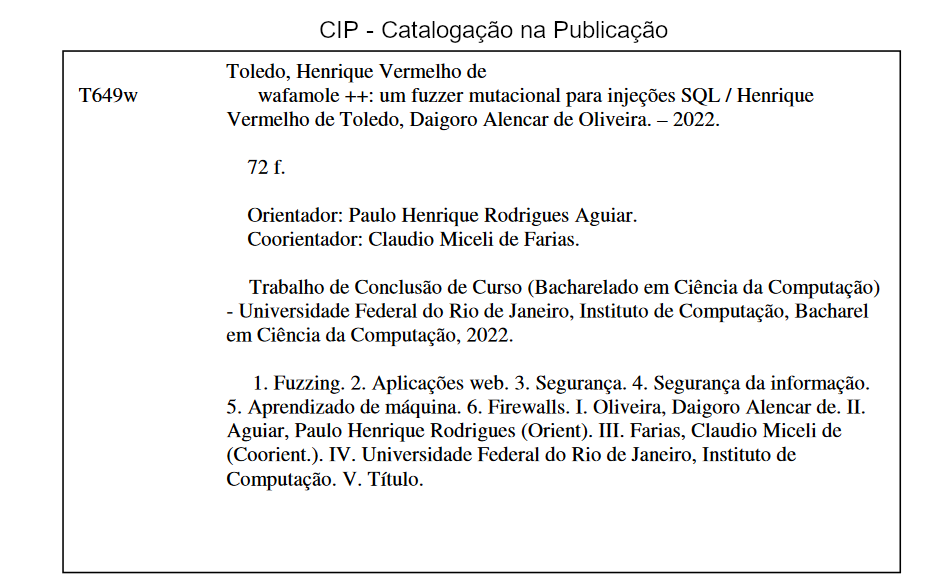
\includegraphics[width=14.217cm,height=9.929cm]{figuras/ficha_cip.png}
\end{figure}
% Opcionalmente você pode usar
% \includepdf{fig_ficha_catalografica.pdf}
\end{fichacatalografica}

%%%%%%%%%%%%%%%%%%%%%%%%%%%%%%%%%%%%%%%%%%%%%%%%%%%%%%%%%
% F O L H A   D E   A P R O V A Ç Ã O  (OBRIGATÓRIO)
%%%%%%%%%%%%%%%%%%%%%%%%%%%%%%%%%%%%%%%%%%%%%%%%%%%%%%%%%
% Isto é um exemplo folha de aprovação.
% Substitua todo o conteúdo desta página por uma
% imagem da página assinada pela banca com o comando abaixo:
% \includepdf{folhadeaprovacao_final.pdf}
%%%%%%%%%%%%%%%%%%%%%%%%%%%%%%%%%%%%%%%%%%%%%%%%%%%%%%%%%

\begin{folhadeaprovacao}
\vspace*{\fill}
\begin{center}
    {\MakeUppercase{\imprimirautor}} 
    \vspace*{\fill}
    \begin{center}
      \imprimirtitulo \\
    \end{center}
    \vspace*{\fill}
  \end{center}
  \hspace*{\fill}\parbox[b]{.5\textwidth}{%
    \linespread{1}\selectfont
    \imprimirpreambulo
}

\vspace*{\fill}
    \begin{flushleft}
 % Alterar a data ou preencher à mão
   Aprovado em \_\_\_ de \_\_\_\_\_\_\_\_\_\_\_\_\_\_ de \_\_\_\_\_\_\_
  \par
  \vspace*{\fill}

BANCA EXAMINADORA:
\end{flushleft}

  \vspace*{\fill}
   \assinatura{Nome do Professor Orientador \\ Titulação (Instituição)}
   \vspace*{\onelineskip}
   \assinatura{Nome do Professor1 \\ Titulação (Instituição)}
   \vspace*{\onelineskip}
   \assinatura{Nome do Professor2\\ Titulação (Instituição)}
   %\assinatura{Nome do Professor, Titulação (Instituição)}
   %\assinatura{Nome do Professor, Titulação (Instituição)}
\vspace*{\fill}
\end{folhadeaprovacao}


%%%%%%%%%%%%%%%%%%%%%%%%%%%%%%%%%%%%%%%%%%%%%%%%%%%%%%%%%%%
% D E D I C A T O R I A  (OPCIONAL)
%%%%%%%%%%%%%%%%%%%%%%%%%%%%%%%%%%%%%%%%%%%%%%%%%%%%%%%%%%%

% \begin{dedicatoria}
\vspace*{\fill}
Dedicatória: Texto no qual o autor do trabalho oferece homenagem ou dedica o seu trabalho a alguém.
\vspace*{\fill}
\end{dedicatoria}

%%%%%%%%%%%%%%%%%%%%%%%%%%%%%%%%%%%%%%%%%%%%%%%%%%%%%%%%%%%%
% A G R A D E C I M E N T O S  (OPCIONAL)
%%%%%%%%%%%%%%%%%%%%%%%%%%%%%%%%%%%%%%%%%%%%%%%%%%%%%%%%%%%% 

\begin{agradecimentos}
Os agradecimentos devem ser dirigidos àqueles que contribuíram de maneira relevante à elaboração do trabalho,
restringindo-se ao mínimo necessário, como instituições (CNPq, CAPES, UFRJ, empresas ou organizações que fizeram parte
da pesquisa), ou pessoas (profissionais, pesquisadores, orientadores, etc.). 

Os agradecimentos devem ser colocados de forma hierárquica de importância e para trabalhos financiados com recursos de
instituições (CAPES, CNPq, FINEP, FAPERJ, etc.) os agradecimentos são obrigatórios a essas instituições.
\end{agradecimentos}

%%%%%%%%%%%%%%%%%%%%%%%%%%%%%%%%%%%%%%%%%%%%%%%%%%%%%%%%%%%%
% E P I G R A F E (OPCIONAL E SEM TÍTULO)
%%%%%%%%%%%%%%%%%%%%%%%%%%%%%%%%%%%%%%%%%%%%%%%%%%%%%%%%%%%% 

% \begin{epigrafe}
\vspace*{\fill}
\begin{flushright}
Epígrafe: É um item onde o autor apresenta a citação de um texto que seja relacionado com o tema do trabalho, seguido da indicação de autoria do mesmo.\\
(texto iniciando do meio da página alinhado à direita)\\
\vspace{\onelineskip}
\textit{‘‘Few are those who see with their \\
own eyes and feel with their own hearts."\\}
\vspace{\onelineskip}
{\bfseries
Albert Einstein 
\par}
(Nome do autor da epígrafe)
\end{flushright}
\end{epigrafe}


%%%%%%%%%%%%%%%%%%%%%%%%%%%%%%%%%%%%%%%%%%%%%%%%%%%%%%%%%%%%
% R E S U M O    E M    P O R T U G U Ê S  (OBRIGATÓRIO)
%%%%%%%%%%%%%%%%%%%%%%%%%%%%%%%%%%%%%%%%%%%%%%%%%%%%%%%%%%%%

\begin{resumo}
\begin{SingleSpace}
Resumo em português. O texto deve ser digitado ou datilografado em um só parágrafo com \textbf{espaçamento simples} e conter de \textbf{150 a 500} palavras. Utilizar a terceira pessoa do singular, os verbos na voz ativa e evitar o uso de símbolos e contrações que não sejam de uso corrente. O resumo deve ressaltar o  objetivo, o método, os resultados e as conclusões do documento. As palavras-chave devem figurar logo abaixo do resumo, antecedidas da expressão \textbf{Palavras-chave:}, separadas por ponto e vírgula (;) e finalizadas por ponto. Devem ser grafadas com as iniciais em letra minúscula, com exceção dos substantivos próprios e nomes científicos.
%separadas entre si por ponto e finalizadas também por ponto.
\end{SingleSpace}
\vspace{\onelineskip}
\textbf{Palavras-chave}: inteligência artificial; criptografia; mineração de dados; Sociedade Brasileira de Computação; redes neurais.
%latex. abntex. editoração de texto.

\end{resumo}

% Palavras-chave separadas e finalizadas por ponto




%%%%%%%%%%%%%%%%%%%%%%%%%%%%%%%%%%%%%%%%%%%%%%%%%%%%%%%%%%%%
% A B S T R A C T  (MANDATORY)
%%%%%%%%%%%%%%%%%%%%%%%%%%%%%%%%%%%%%%%%%%%%%%%%%%%%%%%%%%%%

\begin{resumo}[Abstract]
\begin{otherlanguage*}{english}
\begin{SingleSpace}
Abstract in english. The text should be typed in a single paragraph with \textbf{single spacing} and contain between 150 and 500 words. Use the third person singular, the verbs in the active voice and avoid the use of symbols and contractions that are not of current use. The keywords must appear right below the abstract, preceded by the expression \textbf{Keywords:}, separated by a semicolon (;) and ending with a period. They must be written with the initials in lowercase, with the exception of proper nouns and scientific names.
\end{SingleSpace}

%Eventually you can also write it in spanish \textit{(resumen}), french \textit{(résumé)}, italian \textit{(riassunto)} etc.

\vspace{\onelineskip}
   \textbf{Keywords}: artificial intelligence; cryptography; data mining; Sociedade Brasileira de Computação; neural network.
   
 %  latex. abntex. text editoration.
 \end{otherlanguage*}
\end{resumo}




  


%%%%%%%%%%%%%%%%%%%%%%%%%%%%%%%%%%%%%%%%%%%%%%%%%%%%%%%%%%%%
% L I S T A   D E   I L U S T R A Ç Õ E S  (OPCIONAL)
%%%%%%%%%%%%%%%%%%%%%%%%%%%%%%%%%%%%%%%%%%%%%%%%%%%%%%%%%%%%

\pdfbookmark[0]{\listfigurename}{lof}
\listoffigures*
\cleardoublepage

%%%%%%%%%%%%%%%%%%%%%%%%%%%%%%%%%%%%%%%%%%%%%%%%%%%%%%%%%%%%
% L I S T A   D E   C Ó D I G O S (OPCIONAL)
%%%%%%%%%%%%%%%%%%%%%%%%%%%%%%%%%%%%%%%%%%%%%%%%%%%%%%%%%%%%

\pdfbookmark[0]{\lstlistlistingname}{lol}
\begin{KeepFromToc}
\lstlistoflistings
\end{KeepFromToc}
\cleardoublepage

%%%%%%%%%%%%%%%%%%%%%%%%%%%%%%%%%%%%%%%%%%%%%%%%%%%%%%%%%%%%
% L I S T A   D E   T A B E L A S  (OPCIONAL)
%%%%%%%%%%%%%%%%%%%%%%%%%%%%%%%%%%%%%%%%%%%%%%%%%%%%%%%%%%%%

\pdfbookmark[0]{\listtablename}{lot}
\listoftables*
\cleardoublepage

%%%%%%%%%%%%%%%%%%%%%%%%%%%%%%%%%%%%%%%%%%%%%%%%%%%%%%%%%%%%
% L I S T A   D E   Q U A D R O S (OPCIONAL)
%%%%%%%%%%%%%%%%%%%%%%%%%%%%%%%%%%%%%%%%%%%%%%%%%%%%%%%%%%%%

% \pdfbookmark[0]{\listofquadrosname}{loq}
% \listofquadros*
% \cleardoublepage

%%%%%%%%%%%%%%%%%%%%%%%%%%%%%%%%%%%%%%%%%%%%%%%%%%%%%%%%%%%%
% L I S T A   D E  A B R E V I A T U R A S  E   S I G L A S 
% (OPCIONAL)
%%%%%%%%%%%%%%%%%%%%%%%%%%%%%%%%%%%%%%%%%%%%%%%%%%%%%%%%%%%%

\begin{siglas}
\item[Fig.] Area of the $i^{th}$ component
\item[456] Isto é um número
\item[123] Isto é outro número
\item [Bibliot.] Biblioteconomia
\item [Inform.]  Informática
\item [ABNT] Associação Brasileira de Normas Técnicas
\item [I$^2$C] Inter-Integrated Circuit
\item [SRAM] Static Random-Access Memory
\item [EEPROM]  Electrically Erasable Programmable Read-Only Memory
\item [LED] Light-Emitting Diode
\item [MLP] Modulação por Largura de Pulso
\item [PWM] Pulse-Width Modulation
\item [PID] Proportional–Integral–Derivative
\item [RAM] Random-Access Memory
\item [API] Application Programming Interface
\item [GPL] GNU General Public License
\item [GNU] GNU's Not Unix
\item [iid] Independente e identicamente distribuídas
\end{siglas}

%%%%%%%%%%%%%%%%%%%%%%%%%%%%%%%%%%%%%%%%%%%%%%%%%%%%%%%%%%%%
% L I S T A   D E  S Í M B O L O S   (OPCIONAL)
%%%%%%%%%%%%%%%%%%%%%%%%%%%%%%%%%%%%%%%%%%%%%%%%%%%%%%%%%%%%

% \begin{simbolos}
\item[$ \Gamma $] Letra grega Gama
\item[$ \Lambda $] Lambda
\item[$ \zeta $] Letra grega minúscula zeta
\item[$ \in $] Pertence
\item[\$ ] subcampo
\end{simbolos}

%%%%%%%%%%%%%%%%%%%%%%%%%%%%%%%%%%%%%%%%%%%%%%%%%%%%%%%%%%%%
%  S U M Á R I O  (OBRIGATÓRIO)
%%%%%%%%%%%%%%%%%%%%%%%%%%%%%%%%%%%%%%%%%%%%%%%%%%%%%%%%%%%%
\pdfbookmark[0]{\contentsname}{toc}
\tableofcontents*
\cleardoublepage

%%%%%%%%%%%%%%%%%%%%%%%%%%%%%%%%%%%%%%%%%%%%%%%%%%%%%%%%%%%%
%  E L E M E N T O S   T E X T U A I S  (OBRIGATÓRIO)
%%%%%%%%%%%%%%%%%%%%%%%%%%%%%%%%%%%%%%%%%%%%%%%%%%%%%%%%%%%%
\textual
% Coloca apenas o número da página como cabeçalho
\pagestyle{simple}
\aliaspagestyle{chapter}{simple}

\chapter{INTRODUÇÃO}

Subseções:
* Tema
* 
Discorrer sobre:
* surgimento da internet, 
* evolução de web apps,
* evolução de vulnerabilidades,
* história de defesa de software
* 

O texto deverá ser digitado em espaço 1,5. O parágrafo deverá apresentar um recuo na primeira linha a 1,25cm da margem
esquerda, não contendo espaçamento entre um parágrafo e outro. 

Devem ser digitados em espaços simples: as citações com mais de 3 linhas (citações longas), notas, resumo, referências, legendas de ilustração e de tabelas, bem como partes da capa e da folha de rosto. 

Os títulos das seções devem ser separados do início do texto que os precedem ou os sucedem por um espaço (1,5).

\bigskip


\chapter{REVISÃO DE LITERATURA}
\label{chp:capitulo2}

Em um campo com uma quantia tão rarefeita de artigos, publicações e materiais em larga parte espalhadas por blogs na internet, foi necessário realizar uma revisão de literatura para que as ferramentas de ponta, estratégias ainda sendo testadas e vulnerabilidades principais no mercado fossem corretamente identificadas. Isso se torna especialmente verdadeiro pela mudança no cenário de segurança dos anos 2000 para os anos 2010-2022, aonde boa parte de ameaças antigas podem ser de pouca relevância.

Aqui serão amostrados alguns dos principais achados, as estratégias para organizar os mesmos e resumido o estado da arte no presente momento.

\section{Levantamento de Artigos - Ferramentas empregadas}
\subsection{Parsifal}
Parsifal é uma ferramenta originalmente designada para realizar Revisões Sistemáticas de Literatura, que embora sejam de escopo maior que a revisão rápida que foi realizada neste trabalho, ainda contou com uma série de funcionalidades que permitisse catalogar, processar e essencialmente medir o progresso das pesquisas realizadas no assunto.

\begin{figure}[ht]
    \centering
    \caption{Dashboard Parsifal}
    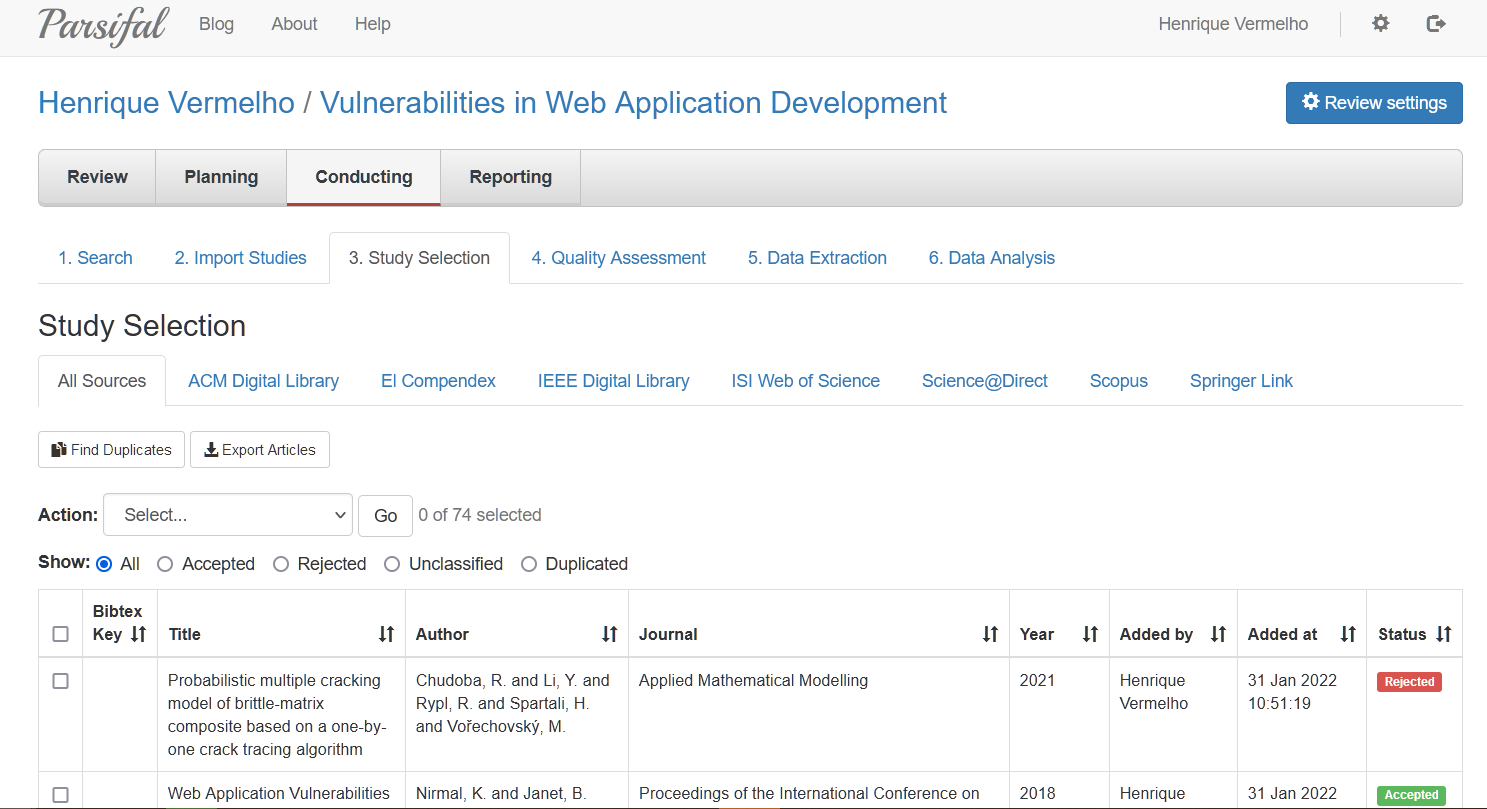
\includegraphics[width=16cm]{figuras/parsifal.png} 
    \legend{Fonte: \href{https://parsif.al}{parsif.al} (2022, p. TO-DO)}
    \label{fig:internet} 
\end{figure}

Na figura acima pode-se verificar no topo quatro abas principais - \textbf{Review, Planning, Conducting, }e \textbf{Reporting}.


\subsection{Scopus + CAFe},
scopus, levantamento de artigos e estado da arte

\section{nscanner}

\section{WAF-A-MoLE}

\subsection{Linear SVM}

\subsection{Seção Terciária}

Alíneas e subalíneas.
\bigskip

\begin{alineas}
\item linha 1:
\begin{alineas}
\item subalinea 1;
\item subalinea 2;
\end{alineas}
\item linha 2:
\begin{subalineas}
\item subalinea 1;
\item subalinea 2;
\end{subalineas}
\item linha 3:
\begin{incisos}
\item subalinea 1;
\item subalinea 2;
\end{incisos}
\item linha 4.
\end{alineas}



\chapter{EMBASAMENTO TEÓRICO}
\label{chp:capitulo3}


SQL injections, Machine Learning utilizado, WAFs, Fuzzing e Algoritmo genetico.

\section{SQL Injection}
Discutir, resumir ponto de partida para assunto na indústria - OWASP top 10.
Artigo respectivo: An OWASP Top Ten Driven Survey on Web
https://owasp.org/www-project-top-ten/

No contexto de segurança das aplicações estudadas, Injeções de código são uma espécie de ataque ocorre quando um atacante testa a segurança de um site enviando dados inesperados para uma aplicação web, fazendo com que a mesma os processe de maneira inválida e se comporte de uma maneira diferente da qual foi originalmente programada. 

O tipo mais comum e mais prevalescente de code injection é o de SQL injection, que manipula bancos de dados via SQL (Structured Query Language), a linguagem clássica de manuseio de bancos de dados, para receber acesso a informações sensíveis.

Exemplificando algumas situações de SQL Injections:

\begin{alineas}
    \item 
    Consideremos uma aplicação que possui uma funcionalidade básica de login, com usuário e senha. Quando o usuário fornece as entradas ‘usuário’ e 123’ como credenciais, a seguinte query SQL é realizada pelo sistema na checagem:
    
    \begin{verbatim}
        SELECT * FROM users 
        WHERE username = ‘usuario’ AND password = ‘123’
    \end{verbatim}
    
    Como a query retorna os detalhes do usuário, o login é bem sucedido. Caso contrário  é rejeitado. Nesse caso, se o atacante usa a sequência de comentário SQL \textbf{--}, ele é capaz de remover a checagem de senha da cláusula \textbf{WHERE}. Exemplificando, se ele submete o usuário \textbf{administrator’--} e uma senha em branco a seguinte query é processada:
    
    \begin{verbatim}
        SELECT * FROM users 
        WHERE username = 'administrator'--' AND password = '' 
    \end{verbatim}
    
    Isso efetivamente retorna o usuário cujo username é administrator e loga o atacante como tal, expondo funções sensíveis da aplicação web inteira.


    
\end{alineas}

\begin{alineas}
    \item
    Em uma aplicação de e-commerce que organiza produtos em categorias diferentes, podemos ter um caso onde o usuário clica em uma categoria de ‘Presentes’, requisitando o seguinte URL do browser:
    
    \textbf{https://insecure-website.com/products?category=Presentes}
    
    Isso faz com que a aplicação realize uma query SQL para resgatar detalhes de tais produtos do banco de dados:
    
    \begin{verbatim}
        SELECT * FROM products
        WHERE category = ‘Presentes' AND released = 1 
    \end{verbatim}
    
    Tal query retorna todos os detalhes (identificado por \textbf{*}) da tabela de produtos, onde a categoria é \textbf{‘Presentes’} e a restrição \textbf{released} é 1. Essa restrição, quando observada por um atacante astuto, se revela como algo usado para esconder produtos não lançados. Esse atacante pode então construir um ataque digitando a seguinte URL, dado que o site não previne contra ataques SQL:
        
    \textbf{https://insecure-website.com/products?category=Presentes’--}
    
    Que provoca a seguinte query SQL:
    
    \begin{verbatim}
        SELECT * FROM products 
        WHERE category = 'Presentes'--' AND released = 1 
    \end{verbatim}
    
     Uma vez que a sequência -- anteriormente vista denota um comentário SQL, a parte depois de 
    ‘Presentes’ é interpretada como tal e não é executada, revelando todos os produtos escondidos.

\end{alineas}

\begin{alineas}
    \item
    Também é possível recuperar dados de outras tabelas de um banco de dados, utilizando a keyword \textbf{UNION}, que combina o resultado de múltiplas consultas \textbf{SELECT} em apenas um conjunto. Se um atacante executa a seguinte query contendo a entrada de usuário \textbf{`Presentes`}, ainda no último exemplo de site:
    
    \begin{verbatim}
        SELECT name, description
        FROM products WHERE category = ‘Presentes'
    \end{verbatim}
    
    Então ele pode também submeter uma entrada nociva com \textbf{UNION}:
    
    \begin{verbatim}
        ' UNION SELECT username, password FROM users--
    \end{verbatim}
        
    Tal entrada faz com que todos os usuários e senhas venham juntos das descrições dos supostos presentes, fundamentalmente comprometendo a segurança da aplicação

\end{alineas}

A prevenção de vulnerabilidades deste tipo são dependentes das tecnologias em uso na aplicação web. Porém, alguns ponteiros básicos podem ser indicados - o uso de uma API segura, que evite o uso do interpretador SQL inteiramente ou use uma interface parametrizada; validação server-side de input positiva ou com “allowlist”; uso de queries LIMIT e outras queries SQL de controle no interpretador para evitar que informações sejam divulgadas em massa. Sumariamente, separar dados da lógica da aplicação web, e implementar configurações e/ou restrições que limitem a exposição dos dados nos casos de code injections bem sucedidas. 

No contexto deste trabalho, no entanto, é estudado uma forma tanto comercial como open-source que têm tido crescimento no mercado: o uso de Web Application Firewalls, mais especificamente o de Web Application Firewalls baseados em técnicas de Machine Learning.

TO-DO: Colocar citações desse trecho de trabFinalMab.pdf 

\section{OWASP TOP 10}

Há pelo menos dez anos os ataques cibernéticos vem aumentando, tendo grande impacto nas empresas.
Aplicações web quando são desenvolvidas sem ter segurança da informação no seu cerne possibilita perda de ativos, inoperabilidade de serviços, exposição de dados sensíveis e comprometimento de sistemas. 
A Open Web Application Security Project (OWASP) é uma fundação sem fins lucrativos cujo objetivo é aprimorar a segurança do software. A organização fornece projeto de código livre, vasta comunidade ativa, conferências, treinamentos e boas práticas. Uma das iniciativas é o OWASP TOP 10, que significa as 10 vulnerabilidades mais comuns:

Injeção;
Broken Authentication;
Broken Access Control;
Design inseguro;
Segurança desconfigurada;
Componentes vulneráveis e desatualizados;
Falhas de identificação e autenticação;
Falhas de integradade de software e dados;
Falhas de monitoramento e security logging;
Server-Side Request Forgery (SSRF).

Injeção
Forma de ataque ampla onde uma entrada de dados recebe caracteres não tratados que são executados pelo sistema com objetivo de alterar o funcionamento padrão do software.
Uma das formas mais conhecidas de injeçao é o SQL Injection. Aplicações vulneráveis a SQL injection geralmente permitem a obtenção completa dos dados do banco de dados e execução de códigos arbitrários remotamente. Existem variantes do SQL Injection como: error-based, union-based, blind e out-of-band. Error-based são injeções que fornecem erros de SQL para o atacante, vazando informações críticas do banco de dados. Union-based são ataques que utilizam uma query existente na lógica do sistema concatenada a outra através de um UNION de maneira a executar uma segunda lógica além da já estabelecida pelo sistema. Injeções às cegas (blind-based) são aquelas que o sistema não dá nenhuma informação após a injeção, de forma que o atacante precisa ser engenhoso para obter informações e prosseguir com a ofensiva. Out-of-band é uma injeção sem o fornecimento de um output para o atacante, porém é possível redirecionar a saída para um endpoint, geralmente servidor http.
É fundamental para mitigar as injeções ter uma validação dos caracteres e declarações válidas ao receber uma entrada de dados na aplicação web.

Broken Authentication


Broken Access Control
Diversos vetores de ataque podem ser considerados Broken access control. Entre eles: burlar verificações de controle de acesso, editar contas de outros usuários, elevação de privilégios, configurações erroneas de CORS (Cross-Origin Resource Sharing) que permitem acesso não autorizado a APIs (Application Programming Interface) restritas, manipulação de metadados através de tokens de controle de acesso JWT (JSON Web Tokens) e acesso não autorizado a páginas web com usuário desprivilegiado, podendo levar ao controle de funções do modelo de negócio ou obtenção de (todos) os dados.
É recomendado ter listas de controle de acesso e negar funcionalidades através de back-end, de forma que o usuário não tem acesso ou controle do código.




TODO:
botar imagem com as top 10 vulnerabilidades
arrumar as referências
verificar acentuação
melhorar listagem de acordo com padrão tcc
verificar se vale a pena deixar alguns termos em ingles tipo broken access control
Organizar subtitulos
No final relacionar injeção com nosso trabalho
Verificar se entrou/saiu algo do owasp moderno
trocar os 2 blogs por livros ou artigos

Referências:

Understanding The Top 10 OWASP Vulnerabilities, Matthew Bach-Nutman
https://arxiv.org/ftp/arxiv/papers/2012/2012.09960.pdf

https://www.indusface.com/blog/10-common-web-application-security-mistakes/
https://www.invicti.com/learn/out-of-band-sql-injection-oob-sqli/
https://owasp.org/www-project-top-ten/

https://d1wqtxts1xzle7.cloudfront.net/37607688/Journal_of_Computer_Science_IJCSIS__Vol._9_No._6_June_2011-with-cover-page-v2.pdf?Expires=1655676531&Signature=FVToQTw7ovULJUkVQdNOpusMs7iq4OGl3gaO2ahUyDDXHTr1NuQC15hcTwL4u4vbHuPF1ROBvFWJ7~vbYsWLc7X~8gT0DtTXxdbevJLOKWnEU9EwDXty0x9MT3Sv-5mo-fkFZrXMyv5k6ePjPEaxNyM8cTkenayq9nSht1A7UuR8iofziF2y0tYmDm9BPNUiUwwz~2qCKXvm4cUS5cJy0NMu2~n3apQOOfX-yg8OSV4sL8tlnYGSyUY7jd73jc-i5T81FaP7JUOcacSLj9g5ZZd5Nh4H-TGBjYWXAtwno32uXchFzxr~6L-fegPDZbWuApnUG2k6rOILf1~cgaQsqQ__&Key-Pair-Id=APKAJLOHF5GGSLRBV4ZA#page=51

\section{Algoritmo Genético}

Explicar mutation rounds, funcionamento de pool e como fuzzer se encaixaria

\section{Algoritmos de Fuzzing}

O cerne do algoritmo por trás do WAF-A-MoLE e o WAF-A-MoLE++ se encontra na técnica de \textit{fuzzing}. O termo fuzz foi cunhado pelo professor da Universidade de Wisconsin-Madison Barton Miller nos anos 80, após sofrer uma interferência considerável de uma tempestade no funcionamento de aplicações que rodavam em um ambiente unix remoto na época. 

Pouco depois disso o mesmo passou aos seus alunos uma tarefa denominada o \textit{"Fuzz Generator"}, na qual era necessário implementar uma ferramenta que testasse a robustez de programas unix através de um bombardeio de informações aleatoriamente geradas.

Atualmente é uma técnica amplamente aceita na testagem/sondagem da segurança de diversas aplicações, com um leque de ofertas de fuzzing comerciais no mercado. E naturalmente é empregável em Web Application Firewalls, permitindo extrair informações valiosas que rendam aprimoramentos para os mesmos.

Uma função elementar de fuzzing, pode ser vista abaixo:

\includecode[C]{Função de um fuzzer elementar} {alg:codigo1}{codigos/fuzzer.py}

\bigskip
Tais funções de fuzzing podem ser aprimoradas, customizadas para testar os mais diversos programas. Uma das maneiras de polir os resultados oriundos de fuzzing elementar, que podem ser rejeitados facilmente por muitos programas inicialmente, é um processo chamado fuzzing mutacional, ou \textit{mutational fuzzing}, projetado para melhorar as chances de obter entradas consideradas válidas.

Nessa estratégia, a execução se inicia com uma entrada válida, e ela subsequentemente sofre uma mutação pequena, como no caso de uma string a mudança de um caractere, adição/remoção de um número, ou até mesmo uma troca de um bit (todos naturalmente aleatórios, pelo princípio do funcionamento de fuzzing).

\includecode[C]{Classe de fuzzer mutacional} {alg:codigo1}{codigos/mutational_fuzzer.py}

\bigskip
O programa acima realiza, dentre 3 operadores de mutação, uma mutação aleatória ao chamar a função mutate(). Na prática, são realizadas uma série de mutações para que se produzam entradas viáveis. Com um simples loop para chamar mutate isso é possibilitado.

O contexto relevante para o WAF-A-MoLE é produzir, iterativamente juntamente com o Algoritmo Genético anteriormente descrito, múltiplas injeções SQL a serem testadas a cada "rodada" de mutação. Uma injeção SQL é usada como base inicial, e a mesma sofre mutações por um fuzzer dedicado até ser considerada válida pelo Web Application Firewall testado, embora seja no fundo ainda uma injeção maliciosa.


Resumidamente, o WAF-A-MoLE++ pode ser descrito como um fuzzer genético, operando em cima de WAFs com entradas "fuzzeadas".

Referências:
https://www.fuzzingbook.org/html/Fuzzer.html
https://www.fuzzingbook.org/html/MutationFuzzer.html
https://fuzzinginfo.wordpress.com/history/

\section{Recurrent Neural Networks}

Para cada um desses, explicar o algoritmo com o funcionamento base, e o funcionamento no Contexto de WAF. Explicar aonde no WAF-A-MoLE entra caso já não tenha sido mencionado. 

\section{Naive Bayes}

\section{Random Forest}

\section{Support Vector Machine}

\subsection{Linear SVM}

\subsection{Gaussian SVM}






Texto.

\subsection{Seção Terciária}

Alíneas e subalíneas.
\bigskip

\begin{alineas}
\item linha 1:
\begin{alineas}
\item subalinea 1;
\item subalinea 2;
\end{alineas}
\item linha 2:
\begin{subalineas}
\item subalinea 1;
\item subalinea 2;
\end{subalineas}
\item linha 3:
\begin{incisos}
\item subalinea 1;
\item subalinea 2;
\end{incisos}
\item linha 4.
\end{alineas}


\section{Exemplo de Tabelas, Quadros e Figuras}

{\centering\bfseries\color{red}
Exemplo de Tabela
\par}

\begin{table}[ht]
\centering
\caption{Preços de alimentos em dólares de 1900-1952 a
1995-1997}
\begin{supertabular}{m{3.6cm}m{3.7cm}m{3.6cm}m{3.0cm}}
\hline
\multicolumn{1}{m{3.636cm}|}{\centering{ ALIMENTO}} &
\multicolumn{1}{m{3.741cm}|}{\centering{ 1950-1952}} &
\multicolumn{1}{m{3.635cm}|}{\centering{ 1995-1977}} &
\centering\arraybslash{ VARIAÇÃO PERCENTUAL}\\\hline
\centering{ Trigo} &
\centering{ 427,6} &
\centering{ 159,3} &
\centering\arraybslash{ {}-62,7}\\
\centering{ Arroz} &
\centering{ 789,7} &
\centering{ 282,3} &
\centering\arraybslash{ {}-64,2}\\
\centering{ Sorgo} &
\centering{ 328,7} &
\centering{ 110,9} &
\centering\arraybslash{ {}-66,2}\\
\centering{ Milho} &
\centering{ 372,0} &
\centering{ 119,1} &
\centering\arraybslash{ {}-68,0}\\\hline
\end{supertabular}
    \legend{Fonte: Sen (2000, p. 240). }
    \label{tab:alimentos}
\end{table}

\bigskip

{\centering\bfseries\color{red}
Exemplo de Quadro
\par}

\begin{quadro}[htb]
\centering
\caption{Comparativo de competitividade}
\begin{supertabular}{|m{2.5cm}|m{2.5cm}|m{6.0cm}|m{3.2cm}|}
\hline
{ EMPRESA } &
{ PRINCIPAL MATÉRIA-PRIMA } &
{ ALTERNATIVAS DE SUPRIMENTOS PARA A PRINCIPAL MATÉRIA-PRIMA } &
{ FLEXIBILIDADE }\\\hline
{ Copesul } &
{ Nafta } &
{ Disponibilidade de produto na Argentina} &
{ 45\% condensado e GLP }\\\hline
{ Copene } &
{ Nafta } &
{ Alternativas Venezuela e Argélia } &
{ Inexistente }\\\hline
{ PQU } &
{ Nafta } &
{ Único fornecedor } &
{ Inexistente }\\\hline
{ Rio Polímeros } &
{ Etano } &
{ Único fornecedor } &
{ Inexistente }\\\hline
{ Baía Blanca } &
{ Etano } &
{ Projeto Mega / Única opção } &
{ Inexistente }\\\hline
\end{supertabular}
    \legend{Fonte: Freire e Jardim (2000, p. 78)}
    \label{quad:quadro1}
\end{quadro}

\bigskip
\clearpage

{\centering\bfseries\color{red}
Exemplo de Gráfico
\par}
\begin{figure}[ht]
    \centering
    \caption{Acesso à internet 1999 – 2002}
    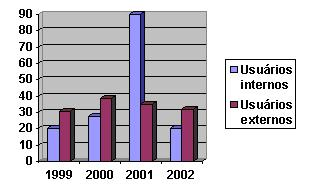
\includegraphics[width=12.5cm,height=7.2cm]{ModeloMonografiaDCCUFRJ-img002.png} 
    \legend{Fonte: Silva, Camargo Pires (2004, p. 45)}
    \label{fig:internet}
\end{figure}


\clearpage
\section{Exemplos de Citações}
{\centering\bfseries\color{red}
Exemplos de Citações
\par}

{\centering\bfseries\color{red}
Citação direta:
\par}

\bigskip

Citações diretas de até 3 linhas, devem iniciar e terminar por aspas duplas.\\

Se o texto original já contiver aspas duplas, substituí-las por aspas simples. A indicação da fonte da citação pode
estar inserida no texto ou após a citação.\\

\bigskip

{\color{red}
Exemplo:}

\bigskip

Segundo Castro (2001, p. 23): {\textquotedbl}Os deveres da conduta do anestesiologista constituem predicados importantes
quando se quer avaliar a qualidade do procedimento.{\textquotedbl}\\

\bigskip

{\color{red}
ou}

\bigskip

{
{\textquotedbl}A expressão 'furiosa' dessa estátua de que fala Rebelais, corresponde também à realidade.{\textquotedbl}
(BAKHTIN, 1987, p. 89).}

\bigskip

{\centering\bfseries\color{red}
Citação Direta com mais de três linhas:
\par}

\bigskip

As citações diretas, no texto, com mais de três linhas, devem ser
destacadas com recuo de 4 cm da margem esquerda, com letra menor que a do texto utilizado e sem as aspas. A indicação da fonte da citação pode estar inserida no texto ou após a citação. \\ 

\bigskip

{\color{red}
Exemplo:}
\bigskip
Sobre mercado financeiro, Fortuna (1996, p. 15) considera:\\
\bigskip

\begin{citacao}
O mercado financeiro permite que um agente econômico qualquer, sem perspectivas de aplicação, em algum empreendimento
próprio, da poupança que é capaz de gerar, seja colocado em contato com outro, cujas perspectivas de investimento
superam as respectivas disponibilidades de poupança.\\
\end{citacao}

\bigskip
A seguir uma citação em inglês:\\

\begin{citacao}[english]
This text is an example in English language in italic with correct hyphenation. This text is an example in English language in italic with correct hyphenation. This text is an example in English language in italic with correct hyphenation.
\end{citacao}
\bigskip

\clearpage{\centering\bfseries\color{red}
Citação Indireta:
\par}

\bigskip

Não se utilizam aspas para esse tipo de citação, nem a(s) página(s) de onde foi extraída a ideia.\\

\bigskip

{\color{red}
Exemplo:}

\bigskip

A bíblia começou a ser escrita no ano 1.000 a.C. e foi finalizada em 100 d.C., com a morte do último apóstolo, São João, levando aproximadamente 1.150 anos para ser concluída \cite{book:GHELLER}.\\


\bigskip

{\centering\bfseries\color{red}
Citação de Citação:
\par}

\bigskip

A indicação da fonte é feita pelo sobrenome do autor da obra citada (não consultada), ano, seguido da expressão latina apud. Após, indica-se o sobrenome do autor da obra consultada, seguido do ano de publicação, precedido por vírgula. Quando for citação direta incluir a(s) página(s) após a data de publicação, precedida de vírgula.\\

\bigskip

{\sffamily
\textrm{\textcolor{red}{Exemplo no texto}}\textrm{:}}

\bigskip

{\sffamily
\textrm{citado por }}

\bigskip

{\sffamily
\textrm{Segundo Marques e Ribeiro}\footnote{\ MARQUES, Alberto; RIBEIRO, \textbf{Angela. As fazendas agrícolas}. São
Paulo: Ática, 2000. 350 p.}\textrm{ (2000 }\textrm{\textcolor{black}{apud }}\textrm{OLIVEIRA, 2001), \apudonline {art:PRADO}{book:AMADO} o Serviço de
Atenção Médico-Sanitário da Suécia tem uma tradição de mais de cem anos. }}

\bigskip

{\color{red}
ou}

{\sffamily
\textrm{\textcolor{red}{Em nota de rodapé}}\textrm{:}}

\bigskip

{\centering\bfseries\color{red}
Indicação da Citação:
\par}

\bigskip

{\sffamily
\textrm{Se a indicação da fonte da citação estiver incluída na frase, a mesma deve aparecer apenas com a inicial
maiúscula seguida de parênteses, com a data de publicação do }\textrm{documento. Quando for citação direta incluir a(s)
página(s) após a data de publicação, precedida de vírgula.}}

\bigskip

{\color{red}
Exemplo com autor pessoal:}

\bigskip

Segundo Fonseca(2004, p. 36): {\textquotedbl}Se não houver mecanismos jurídicos que assegurem a proteção dos direitos
humanos, esse valor não será concretizado pelo Poder Público.{\textquotedbl}\\

\bigskip

{\sffamily
\textrm{\textcolor{red}{Exemplo com dois autores: }}}

\bigskip

Tonetto e Reck (2001, p. 134) destacam: {\textquotedbl}Este autoconhecimento pressupõe conhecer seus limites
[...]{\textquotedbl} \\

\bigskip

{\color{red}
Exemplo com mais de três autores:}

\bigskip

Neste contexto, Couto e outros (2004, p. 52) destacam que: {\textquotedbl}No capitalismo não é a simples ausência do
patrão que promove a superação do despotismo da divisão laboral.{\textquotedbl}\\

\bigskip

{\sffamily
\textrm{\textcolor{red}{Exemplo com autor institucional: }}}

\bigskip

De acordo com a Pontifícia Universidade Católica do Rio Grande do Sul (2001, p. 24): {\textquotedbl}[...] no horizonte 2001/2010, o esforço estratégico da PUCRS será centrado em sete áreas estratégicas [...]{\textquotedbl}\\

\bigskip

{\color{red}
Exemplo sem autor(es), com a entrada pelo título:}

\bigskip

Segundo o Guia de clareamento dental (1996, p. 8): {\textquotedbl}A causa mais comum do escurecimento dental é o tratamento endodôntico realizado de modo inadequado e sem os cuidados técnicos.{\textquotedbl}\\

\bigskip

{\color{red}
Exemplo sem autor(es), com a entrada pelo título que inicia por artigo:}

\bigskip

O movimento social, com o intuito de realizar uma transformação social, é uma das tarefas mais importantes da atualidade
(O COOPERATIVISMO..., 2002).\\

\bigskip

As citações a seguir foram colocadas para que as referências aparecessem na bibliografia. Como exemplo temos os livro de Jorge Amado \cite{book:AMADO}  \cite{book:AMADO2}, e este autor que desconheço \cite{book:OHANSSON}, além de \cite{book:ENGEL} e um artigo \cite{art:PRADO}. Notem que é gerado um link hipertexto no documento em PDF.


\chapter{WAF-A-MoLE++}
\label{chp:capitulo4}

\section{Estruturação do Projeto}

\section{WAFs avaliados}

\subsection{WAF-Brain}

\textbf{Autores}: Sergio D Fdez, cr0hn, Enrique Garcia. Disponível no Github \href{https://github.com/BBVA}{BBVA}

O WAF-Brain foi um dos primeiros firewalls a serem testados pela equipe do WAF-A-MoLE, e subsequentemente é o primeiro modelo de exemplo disponibilizado para testes na documentação do mesmo. Dessa maneira, foi extensivamente testado com os novos operadores de mutação, sendo de grande ajuda para diagnosticar os incluídos no WAF-A-MoLE++.

\begin{figure}[ht]
    \centering
    \caption{Dependências e logomarca do WAF-Brain}
    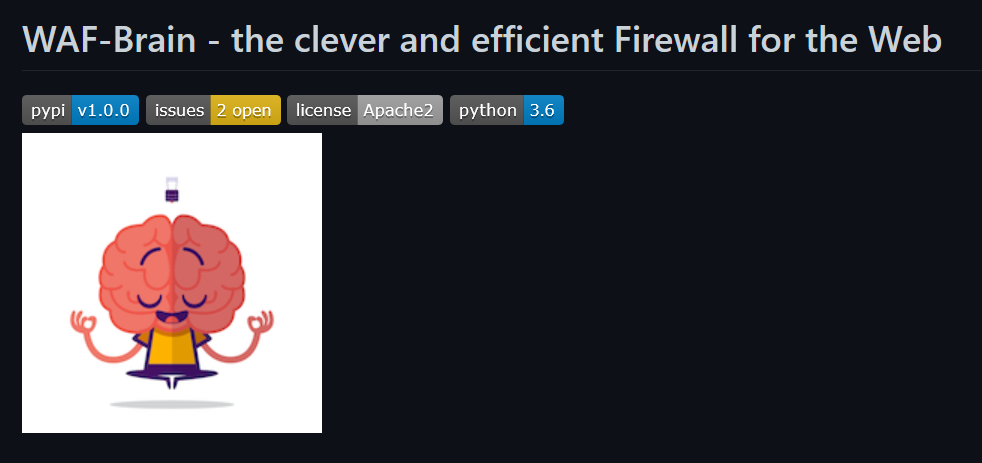
\includegraphics[width=12.5cm]{figuras/WAFBrain.png} 
    \legend{Fonte: \href{https://github.com/BBVA}{Github} (2019, p. TO-DO)}
    \label{fig:internet} 
\end{figure}

Seu funcionamento se dá, como anteriormente mencionado, através da estratégia de Deep Learning com Redes Neurais, pela qual são analisados cada campo de um determinado pedido HTTP sob a ótica de um classificador treinado desta maneira, determinando se esse campo é malicioso ou não.

Na adaptação WAF-A-MoLE, esse poder de predição é aproveitado exclusivamente na forma de probabilidade - tendo a probabilidade de ser uma SQL-Injection acima de um determinado limite, temos um caso malicioso. Isso requer que o classificador treinado no modelo não apenas mostre a previsão, mas também a precisa probabilidade com a qual chegou à mesma.

Por mais que se trate de um algoritmo sofisticado por natureza, surpreendentemente o WAF-Brain fora implementado pelos seus autores originais de uma maneira simplória o suficiente para ser um dos WAFs mais vulneráveis às estratégias de fuzzing do WAF-A-MoLE. Vários operadores de mutação isolados conseguem resultados frutíferos em pouco tempo, como será visto na seção de testes adiante.

\section{Operadores de Mutação}

\section{Modelos}
Todos os modelos implementados tiveram como base o firewall ML-Based-WAF, disponível por vladan-stojnic no \href{https://github.com/vladan-stojnic/ML-based-WAF}{Github} que fora o WAF open source mais promissor e mais plausível de adaptar. Sua performance também era factível no contexto de recursos disponíveis para a conclusão deste projeto final.

\begin{figure}[ht]
    \centering
    \caption{Repositório ML-Based-WAF}
    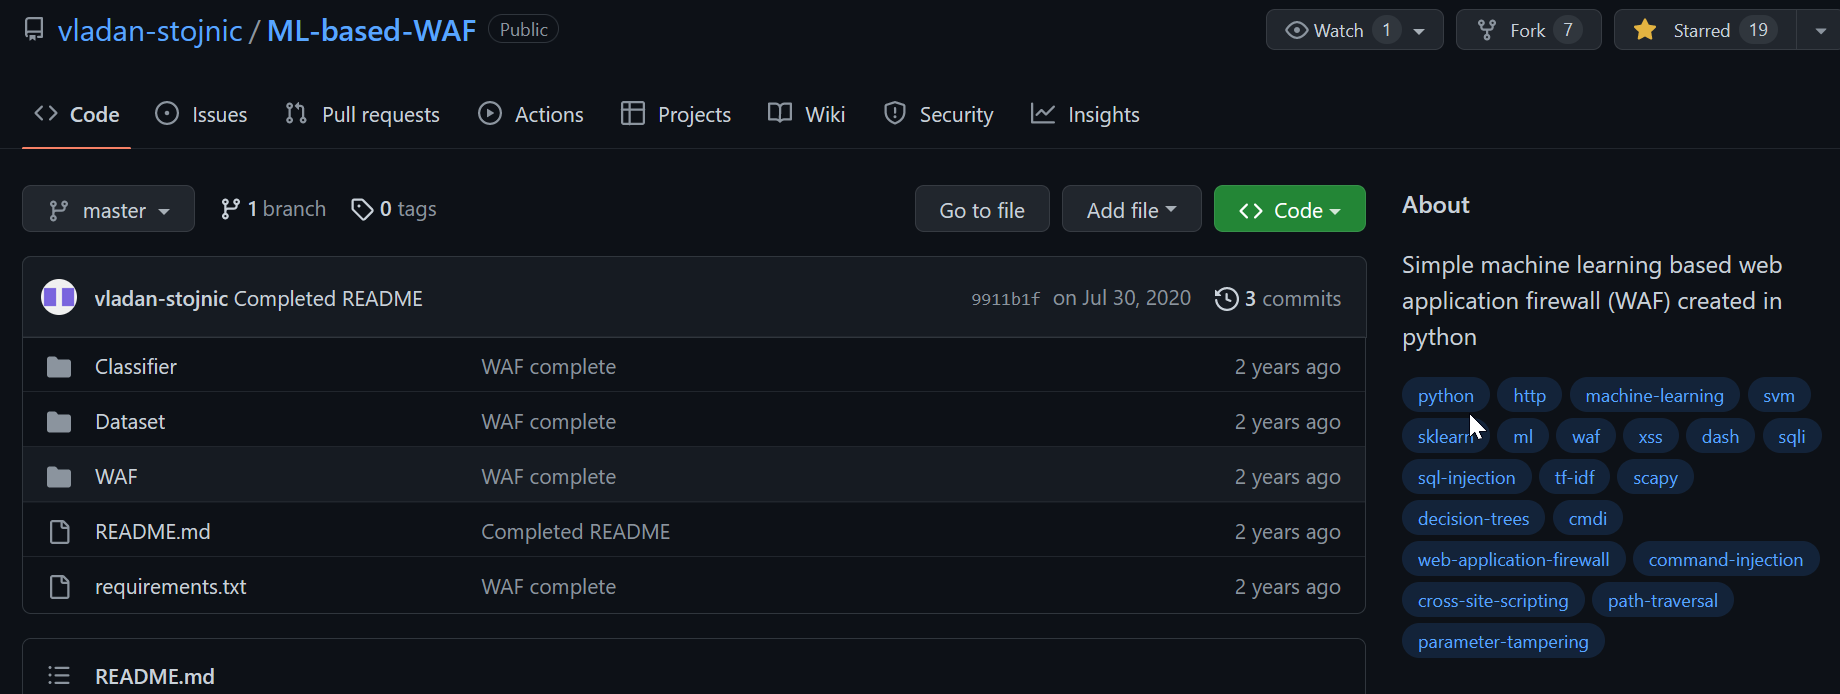
\includegraphics[width=16cm]{figuras/MLBasedWAF.png} 
    \legend{Fonte: \href{https://github.com/vladan-stojnic/ML-based-WAF}{Github} (2020, p. TO-DO)}
    \label{fig:internet} 
\end{figure}

Embora seja um WAF orientado ao tráfego real ou simulado de uma rede de fato, avaliando parâmetros HTTP em tempo real no seu componente sniffer.py tanto por SQL-Injections como por outras formas de ataque (XSS, cmdi e outras), ainda foi possível restringir seu funcionamento para adaptá-lo ao WAF-A-MoLE++. 

Para tal, foi necessário prever uma estratégia própria de treinamento para o classificador, além de um conjunto de dados especial para o mesmo. É cabível mencionar, no entanto, que isso introduziu uma série de dificuldades uma vez que sua documentação era consideravelmente modesta, e o banco novo a ser usado deveria seguir o padrão de formatação seguido pelo WAF.

Dentre as opções de datasets disponíveis com SQL Injections, foi escolhido inicialmente a versão SQLiV3.json da coleção do Kaggle que será amostrada a seguir.
Além disso, para corrigir uma variedade de erros de formatação, polir algumas queries incorretas (e de difícil proveito), e finalmente adaptar para o padrão .json utilizado pelo WAF, a seguinte função auxiliar foi codificada:

\begin{figure}[ht]
    \centering
    \caption{Detalhes Dataset SQL Injection Kaggle.}
    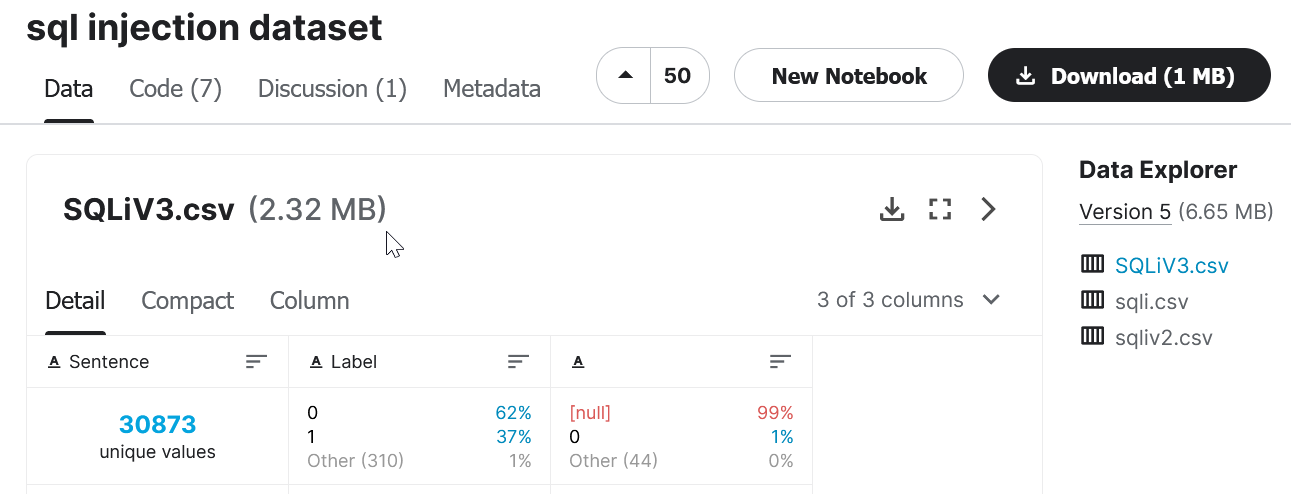
\includegraphics[width=16cm]{figuras/sqlInjectionDataset.png} 
    \legend{Fonte: \href{https://www.kaggle.com/datasets/syedsaqlainhussain/sql-injection-dataset}{Kaggle} (2021, p. TO-DO)}
    \label{fig:internet} 
\end{figure}

\label{sec:codigos}
\includecode[C]{Para tratamento de dados brutos} {alg:codigo3}{codigos/sqli_cleaner.py}

\subsection{Support Vector Machine}
Este foi o primeiro modelo implementado no WAF-A-MoLE++, antes do recebimento do dataset original da equipe original. 







\chapter{PROJETO DE TESTES REALIZADO}
\label{chp:capitulo5}

\section{Equações}
\label{sec:equacoes}
Referência: \url{http://en.wikibooks.org/wiki/LaTeX/Mathematics}

Também: \url{http://en.wikibooks.org/wiki/LaTeX/Advanced_Mathematics}

\begin{equation}
  (x + y)^2 = x^2 + 2xy + y^2
  \label{eq:equacao1}
\end{equation}

\section{Códigos}
\label{sec:codigos}
Reference: \url{http://en.wikibooks.org/wiki/LaTeX/Source_Code_Listings}

%\includecode[Linguagem]{Caption}{Label}{Arquivo}
\includecode[C]{Exemplo em Linguagem C} {alg:codigo1}{codigos/codigo.c}

%\includecode[Linguagem]{Caption}{Label}{Arquivo}
\includecode[Java]{Exemplo em Linguagem Java} {alg:codigo2}{codigos/codigo.java}

\section{Referências}
\label{sec:referencias}

A seguir como referenciar da maneira correta capítulos, seções, tabelas, etc. no texto corretamente.\\

\begin{itemize}
  \item Capítulo \ref{chp:capitulo4}
  \item Seção \ref{sec:codigos}
  \item Seção \ref{sec:referencias}
  \item Tabela \ref{tab:alimentos}
  \item Quadro \ref{quad:quadro1}
  \item Figura \ref{fig:internet}
  \item Equação \ref{eq:equacao1}
  \item Código \ref{alg:codigo1}
\end{itemize}

Para produzir um glossário em \Gls{latex} utilize o comando \emph{$\backslash$gls\{termo\}} para incluir a referência a um termo do glossário no texto. Um link de hipertexto será criado automaticamente para o termo no glossário como em \gls{maths}. 

As \glspl{formula} são processadas adequadamente e facilmente uma vez que o usuário se acostuma com os comandos. 
 
Dado um conjunto de números, há métodos elementares para calcular o seu \acrlong{mdc}, que é abreviado \acrshort{mdc}. Este processo é similar ao utilizado para o  \acrfull{mmc}.

Veja o arquivo glossario.tex em anexo para alguns exemplos simples.



\chapter{CONSIDERAÇÕES FINAIS}
\label{chp:capitulo6}


Onde se expõe o fechamento das ideias do estudo, são apresentados os resultados da pesquisa, e partindo da análise destes resultados, tiram-se as conclusões e se for necessário, as sugestões relativas ao estudo. \\

Observação: É opcional a apresentação dos desdobramentos relativos à importância, síntese, projeção, repercussão, encaminhamento e outros.


\postextual
%%%%%%%%%%%%%%%%%%%%%%%%%%%%%%%%%%%%%%%%%%%%%%%%%%%%
% R E F E R Ê N C I A S  (OBRIGATÓRIO)
%%%%%%%%%%%%%%%%%%%%%%%%%%%%%%%%%%%%%%%%%%%%%%%%%%%%

\bibliography{elementos-postextuais/referencias.bib}

%%%%%%%%%%%%%%%%%%%%%%%%%%%%%%%%%%%%%%%%%%%%%%%%%%%%
% G L O S S A R I O (opcional)
%%%%%%%%%%%%%%%%%%%%%%%%%%%%%%%%%%%%%%%%%%%%%%%%%%%%
% \clearpage
% \addcontentsline{toc}{chapter}{GLOSSÁRIO} %\glossaryname
% \printglossary

%%%%%%%%%%%%%%%%%%%%%%%%%%%%%%%%%%%%%%%%%%%%%%%%%%%%%%%%%
% A P Ê N D I C E S  (Opcional) 
%%%%%%%%%%%%%%%%%%%%%%%%%%%%%%%%%%%%%%%%%%%%%%%%%%%%%%%%%
%\textrm{\textcolor{red}{Apêndice(s) (Este item é elaborado 
% pelo próprio autor do trabalho e serve para  complementar
% a sua argumentação.  É um elemento \textbf{opcional)}.}}
%%%%%%%%%%%%%%%%%%%%%%%%%%%%%%%%%%%%%%%%%%%%%%%%%%%%%%%%

\clearpage
\begin{apendicesenv}

\begin{vplace}
{\centering
\ABNTEXchapterfont{\textrm{APÊNDICES}}
\par}
\end{vplace}
\newpage
{\let\clearpage\relax \chapter{\textnormal{Análise dos
relatórios mensais de uso do serviço de renovação de empréstimos.}}}

Lorem ipsum dolor sit amet, consectetur adipiscing elit. Donec lacus nisl, ultricies vitae semper eu, scelerisque nec enim. Curabitur posuere tortor orci, at porta leo laoreet et. Quisque ut congue dolor. Maecenas vel sagittis diam. Praesent fermentum eleifend mi, sit amet vehicula leo pellentesque quis. Curabitur mattis luctus pulvinar. Proin auctor est nec nulla pellentesque commodo. Donec nec justo eu magna aliquet eleifend. Curabitur tristique tortor id sem dignissim, a iaculis metus interdum. Phasellus bibendum velit sit amet interdum semper. Nam vestibulum dui quis nisi consectetur, id vehicula dolor faucibus.\\
\newpage
{\let\clearpage\relax \chapter{\textnormal{Análise dos
relatórios mensais de uso do serviço de empréstimo domiciliar.}}}

Lorem ipsum dolor sit amet, consectetur adipiscing elit. Donec lacus nisl, ultricies vitae semper eu, scelerisque nec enim. Curabitur posuere tortor orci, at porta leo laoreet et. Quisque ut congue dolor. Maecenas vel sagittis diam. Praesent fermentum eleifend mi, sit amet vehicula leo pellentesque quis. Curabitur mattis luctus pulvinar. Proin auctor est nec nulla pellentesque commodo. Donec nec justo eu magna aliquet eleifend. Curabitur tristique tortor id sem dignissim, a iaculis metus interdum. Phasellus bibendum velit sit amet interdum semper. Nam vestibulum dui quis nisi consectetur, id vehicula dolor faucibus.\\
\newpage
% {\let\clearpage\relax \chapter{\textnormal{Lista de Operadores de Mutação}}}

% \begin{figure}[ht]
%     \centering
%     \caption{Lista de operadores de mutação WAF-A-MoLE}
%     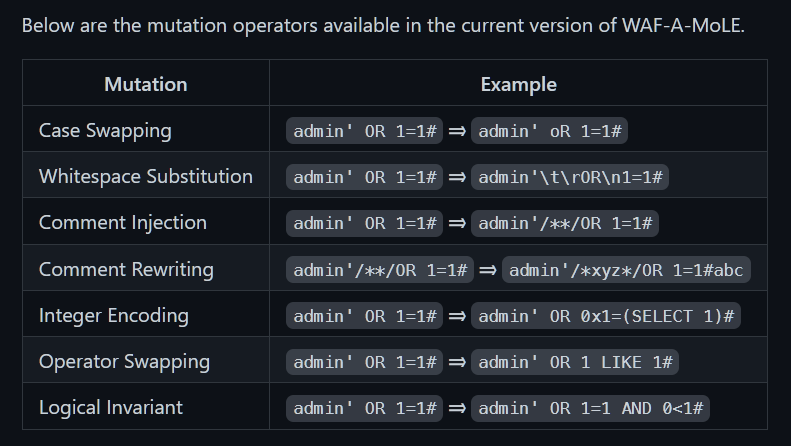
\includegraphics[width=16cm]{figuras/mutation_operators_wafamole.png}
%     \legend{Fonte: WAF-A-MoLE GitHub (2022)}
%     \label{fig:internet} 
% \end{figure}
\end{apendicesenv}

%%%%%%%%%%%%%%%%%%%%%%%%%%%%%%%%%%%%%%%%%%%%%%%%%%%%%%%%%
% A N E X O S   (Opcional) 
%%%%%%%%%%%%%%%%%%%%%%%%%%%%%%%%%%%%%%%%%%%%%%%%%%%%%%%%%
% \textrm{\textcolor{red}{Anexos (Este item é constituído por 
% documentos complementares ao texto do trabalho e que não são 
% elaborados pelo autor do mesmo, servem para fundamentação, 
% comprovação e ilustração. É um elemento \textbf{opcional}).}}
%%%%%%%%%%%%%%%%%%%%%%%%%%%%%%%%%%%%%%%%%%%%%%%%%%%%%%%%%

% \clearpage
% \begin{anexosenv}

% \begin{vplace}
% {\centering
% \ABNTEXchapterfont{ANEXOS}
% \par}
% \end{vplace}
% \newpage
% {\let\clearpage\relax \chapter{\textnormal{Demonstrativo de
frequência diária ago./set. 2001}}}

Lorem ipsum dolor sit amet, consectetur adipiscing elit. Donec lacus nisl, ultricies vitae semper eu, scelerisque nec enim. Curabitur posuere tortor orci, at porta leo laoreet et. Quisque ut congue dolor. Maecenas vel sagittis diam. Praesent fermentum eleifend mi, sit amet vehicula leo pellentesque quis. Curabitur mattis luctus pulvinar. Proin auctor est nec nulla pellentesque commodo. Donec nec justo eu magna aliquet eleifend. Curabitur tristique tortor id sem dignissim, a iaculis metus interdum. Phasellus bibendum velit sit amet interdum semper. Nam vestibulum dui quis nisi consectetur, id vehicula dolor faucibus.\\
% \newpage
% {\let\clearpage\relax \chapter{\textnormal{Demonstrativo de frequência diária jan./dez. 2002}}}

Lorem ipsum dolor sit amet, consectetur adipiscing elit. Donec lacus nisl, ultricies vitae semper eu, scelerisque nec enim. Curabitur posuere tortor orci, at porta leo laoreet et. Quisque ut congue dolor. Maecenas vel sagittis diam. Praesent fermentum eleifend mi, sit amet vehicula leo pellentesque quis. Curabitur mattis luctus pulvinar. Proin auctor est nec nulla pellentesque commodo. Donec nec justo eu magna aliquet eleifend. Curabitur tristique tortor id sem dignissim, a iaculis metus interdum. Phasellus bibendum velit sit amet interdum semper. Nam vestibulum dui quis nisi consectetur, id vehicula dolor faucibus. \\

% \end{anexosenv}

%%%%%%%%%%%%%%%%%%%%%%%%%%%%%%%%%%%%%%%%%%%%%%%%%%%%%%%%%
% F I M   D O  D O C U M E N T O
%%%%%%%%%%%%%%%%%%%%%%%%%%%%%%%%%%%%%%%%%%%%%%%%%%%%%%%%%
\end{document}